% Chapter 3: Thiết kế phần cứng bộ điều khiển bay
\chapter{Thiết kế phần cứng bộ điều khiển bay}

Chương này trình bày quá trình phát triển phần cứng của bộ điều khiển bay \textbf{FC-v01}. Phần cứng được thiết kế gồm hai phiên bản bản mạch in (printed circuit board, PCB), trong đó phiên bản v2 đang được nhóm sử dụng. Nội dung gồm tổng quan bản mạch, khối xử lý trung tâm, hệ thống cấp nguồn và bảo vệ, cùng các khối cảm biến -- ngoại vi.

\section{Tổng quan bản mạch}

Bản mạch có kích thước $50 \times 50$~mm và bốn lớp đồng (bốn lớp mạch dẫn điện xếp chồng). Bốn lỗ bắt vít M3 ở bốn góc theo khoảng cách $42 \times 42$~mm, nên tương thích trực tiếp (drop-in) với khung quadcopter (máy bay bốn động cơ) phổ thông. Phiên bản v1 xác nhận mô hình ``bảng mang'' (carrier board): các mô-đun cảm biến thương mại gắn trên một bảng mạch thiết kế riêng, tối ưu chi phí mà vẫn bảo đảm chất lượng tín hiệu. Phiên bản v2 khắc phục hạn chế về bố trí dây dẫn và kết nối của v1, tách riêng đường nguồn cảm biến +3V3\_SENS và được dùng trong mọi thí nghiệm của báo cáo. Hình~\ref{fig:fc-renders} trình bày mặt trước và mặt sau của bản mạch v2.

\begin{figure}[h]
\centering
\begin{minipage}{0.44\textwidth}
\centering
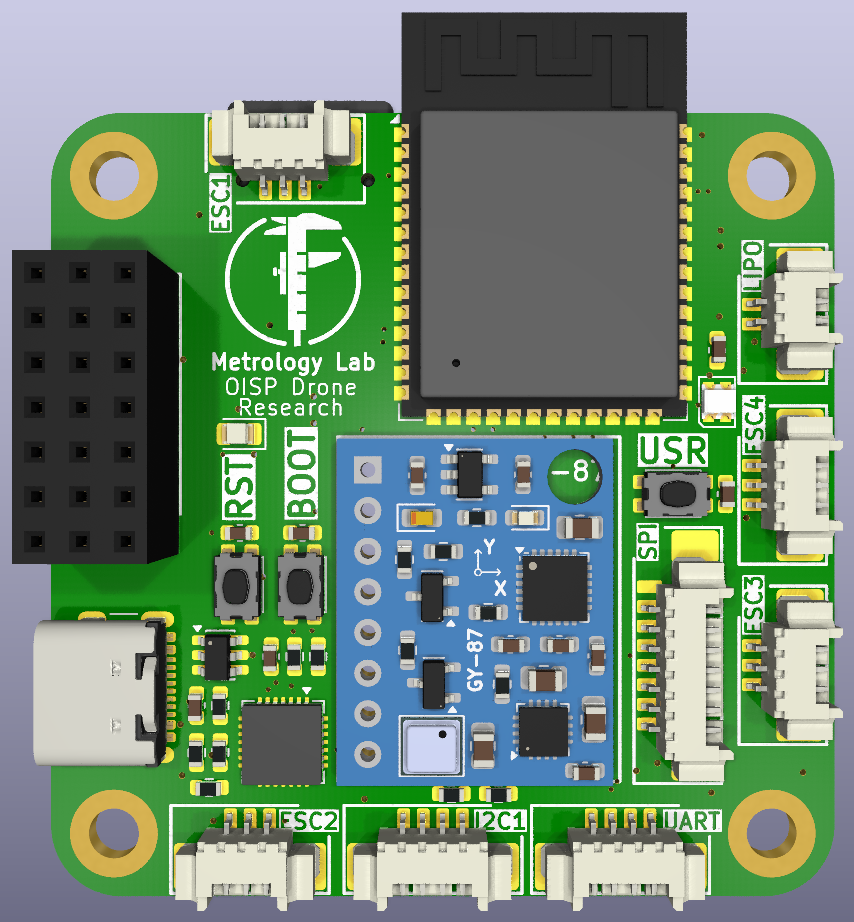
\includegraphics[width=\linewidth]{imgs/fc_v02_front.png}\\[2pt]
(a) Mặt trước
\end{minipage}
\hfill
\begin{minipage}{0.44\textwidth}
\centering
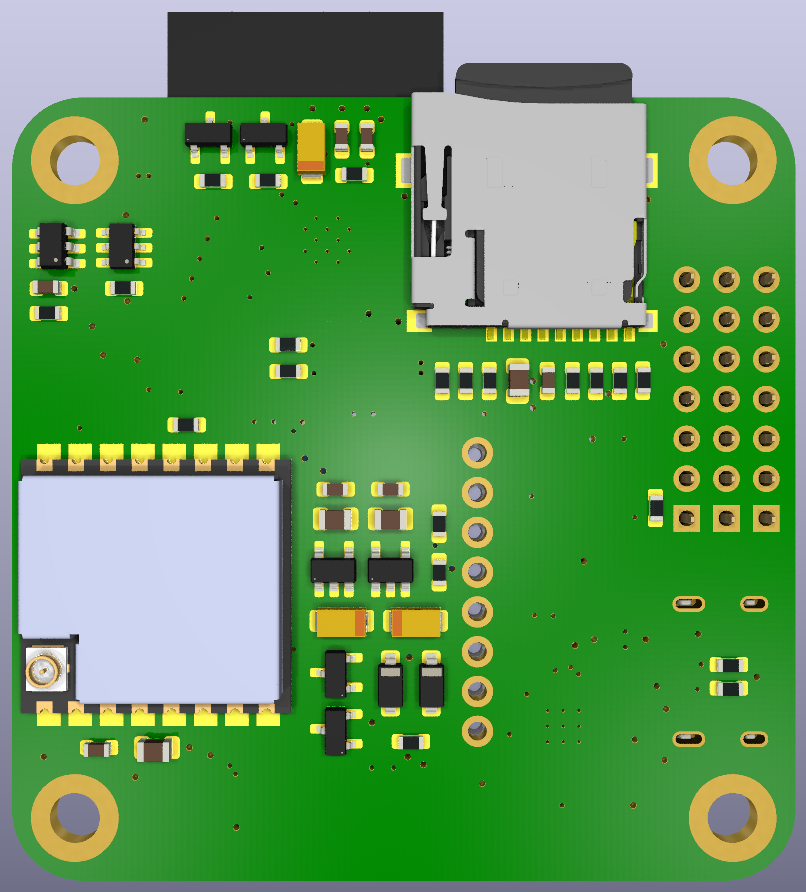
\includegraphics[width=\linewidth]{imgs/fc_v02_back.png}\\[2pt]
(b) Mặt sau
\end{minipage}
\caption{Kết xuất 3D bản mạch \textbf{FC-v01} phiên bản v2: mặt trước chứa ESP32-S3-WROOM-1, mô-đun GY-87, cổng USB-C, các connector ESC và header máy thu; mặt sau chứa khe thẻ microSD và mô-đun vô tuyến dự trữ.}
\label{fig:fc-renders}
\end{figure}

\section{Khối xử lý trung tâm}

Bộ điều khiển trung tâm là mô-đun ESP32-S3-WROOM-1-N8-R8 của Espressif~\cite{wroom} (hình~\ref{fig:esp32s3}). ESP32-S3 là vi điều khiển (chip tính toán cho mục đích điều khiển). Mô-đun dùng vi điều khiển hai nhân Xtensa LX7 ở 240~MHz, bộ nhớ flash 8~MB và bộ nhớ PSRAM (RAM tĩnh giả ngoài chip) 8~MB. Lý do chọn: (1) hai nhân xử lý đủ tải cho chuỗi thu nhận -- tiền xử lý -- ước lượng trạng thái 500~Hz; (2) PSRAM cho phép cấp phát tĩnh các bộ đệm lớn ghi dữ liệu bay; và (3) hệ thống ngoại vi phong phú (LEDC, RMT, nhiều bộ SPI/I\textsuperscript{2}C độc lập) cho mỗi khối chức năng một kênh phần cứng riêng~\cite{trm}.

\begin{figure}[h]
\centering
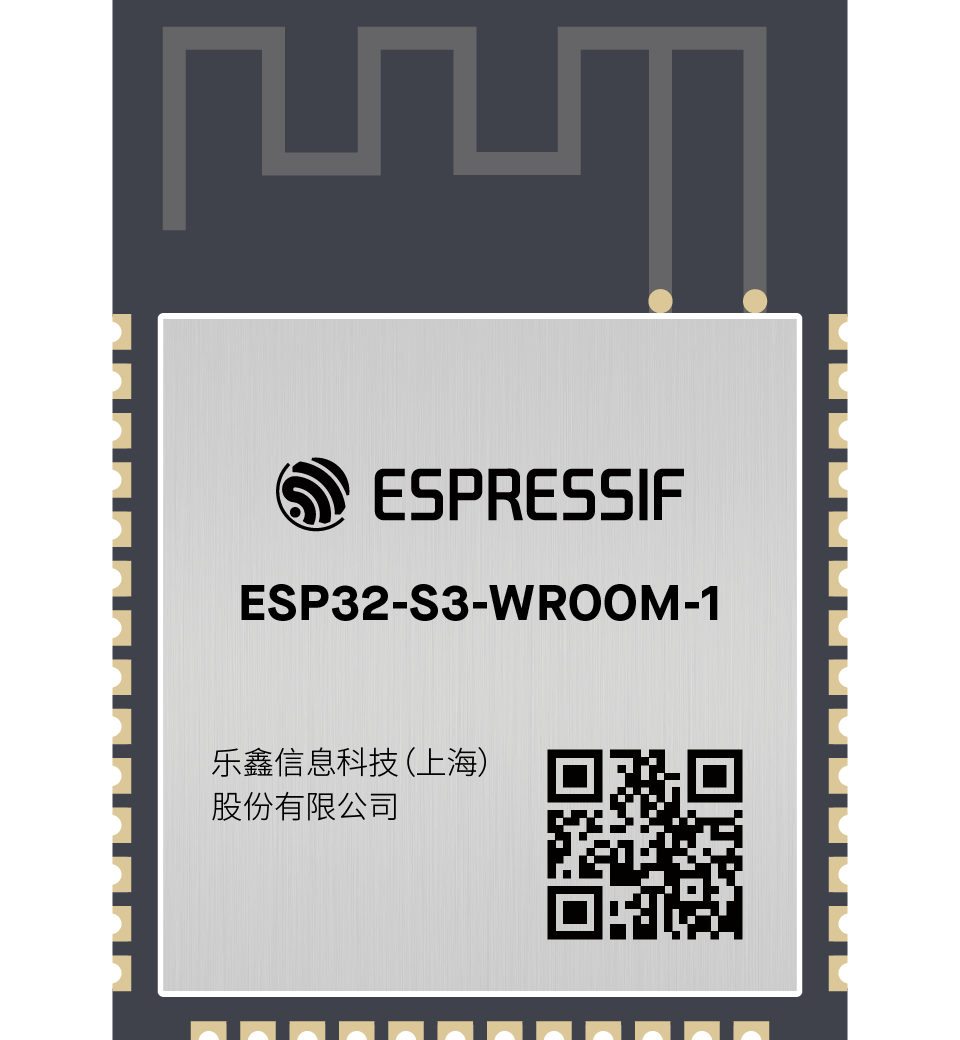
\includegraphics[width=0.30\textwidth]{imgs/esp32s3_wroom1.png}
\caption{Mô-đun ESP32-S3-WROOM-1 (Nguồn: Espressif Systems).}
\label{fig:esp32s3}
\end{figure}

Bảng~\ref{tab:periph} tổng hợp phân bổ ngoại vi của bản mạch v2. Bốn kênh PWM (điều chế độ rộng xung -- cách điều khiển bằng độ rộng của xung điện) cho ESC (electronic speed controller, khối điều khiển tốc độ động cơ) được tạo bằng timer LEDC ở tần số 250~Hz, độ phân giải 14~bit, xung 1000--2000~µs theo giao thức truyền thống. Máy thu FlySky FS-iA6B nối qua header 7 chân (GND và sáu kênh tín hiệu); tín hiệu PPM (ghép nhiều kênh điều khiển trên một dây) sáu kênh được giải mã bằng RMT (khối phần cứng ESP32 tạo và đo dãy xung) ở GPIO~5. Đèn trạng thái WS2812B và nút người dùng lần lượt dùng GPIO~2 và GPIO~38.

\begin{table}[h]
\centering
\caption{Phân bổ ngoại vi của bản mạch \textbf{FC-v01} v2}
\label{tab:periph}
\footnotesize
\begin{tabular}{p{3.2cm}p{5.0cm}p{6.2cm}}
\toprule
Ngoại vi & Chức năng & Cấu hình \\
\midrule
LEDC (4 kênh) & Xuất PWM điều khiển ESC & 250~Hz, 14 bit, xung 1000--2000~µs; GPIO 4/3/40/1 \\
I\textsuperscript{2}C0 & GY-87 (MPU6050, HMC5883L, BMP180) & 400~kHz; SDA GPIO~21, SCL GPIO~14 \\
SPI -- thẻ microSD & Ghi dữ liệu bay (blackbox) & CS GPIO~8, phát hiện thẻ GPIO~18 \\
SPI -- vô tuyến & Kết nối mô-đun RA-02 (dự trữ) & CS GPIO~39, RST GPIO~41; chưa tích hợp driver \\
RMT (RX) & Giải mã PPM máy thu FS-iA6B & 6 kênh; GPIO~5 \\
RMT (TX) & LED trạng thái WS2812B & GPIO~2 \\
USB-UART (CP2102) & Nạp firmware, giám sát qua USB-C & DTR/RTS tự reset vào chế độ boot \\
UART & Dự trữ (GNSS) & GPIO 9/10 \\
USB-Serial-JTAG & Gỡ lỗi, JTAG hai dây & GPIO 19/20 (chia sẻ I\textsuperscript{2}C1 dự trữ) \\
\bottomrule
\end{tabular}
\end{table}

\section{Cấp nguồn và bảo vệ}

Bản mạch v2 có ba nguồn vào: (1) chân BEC trên connector ESC (ESC truyền thống tích hợp mạch loại bỏ pin -- battery elimination circuit -- xuất nguồn 5~V); (2) pin LiPo 1S qua connector JST; và (3) cổng USB Type-C. Khi bay, bộ điều khiển lấy nguồn từ BEC của ESC; trên bàn phát triển, hệ thống chạy chủ yếu từ USB và pin 1S. Ba nguồn được trộn tự động bằng diode OR (loại 1N5819, linh kiện chỉ cho dòng đi một chiều -- chọn nguồn cao hơn) cùng công tắc tải (load switch) SI2301: nguồn cao hơn ưu tiên cấp mà không gây dòng ngược.

Nguồn 5~V được ổn áp thành hai đường 3,3~V độc lập. Bộ ổn áp tuyến tính (LDO) ME6211C33 cấp đường +3V3\_SENS \emph{riêng} cho mô-đun GY-87, gồm ba mạch con MPU6050, HMC5883L và BMP180. LDO AP2112K-3.3 cấp đường +3V3 chính cho toàn bộ các khối còn lại, kể cả khối xử lý trung tâm. Việc tách riêng này hạn chế nhiễu xung chuyển mạch (gợn nhiễu khi mạch số đóng ngắt dòng nhanh) từ các khối còn lại lan sang chân nguồn cảm biến -- quan trọng với cảm biến áp suất có biên độ nhiễu lớn (được phân tích ở chương ước lượng trạng thái).

Khối bảo vệ pin Li-Ion 1S (DW01A kết hợp cặp MOSFET FS8205, hai linh kiện bán dẫn đóng ngắt dòng) ngăn xả quá mức, sạc quá mức và quá tải cho pin cấp qua connector JST; khối này phục vụ nghiên cứu trên bàn thí nghiệm, không thuộc đường cấp nguồn khi bay.

\section{Cảm biến và ngoại vi}

Cảm biến quán tính -- từ tính -- áp suất của hệ thống là mô-đun GY-87 (hình~\ref{fig:gy87}), gồm MPU6050~\cite{mpu6050} (gia tốc kế, con quay hồi tiếp), HMC5883L~\cite{hmc5883l} (từ kế, đo từ trường; nối qua cơ chế bypass I\textsuperscript{2}C của MPU6050) và BMP180~\cite{bmp180} (cảm biến áp suất). Mô-đun được gắn trực tiếp lên bản mạch qua header, trên đường nguồn cảm biến +3V3\_SENS độc lập.

\begin{figure}[H]
\centering
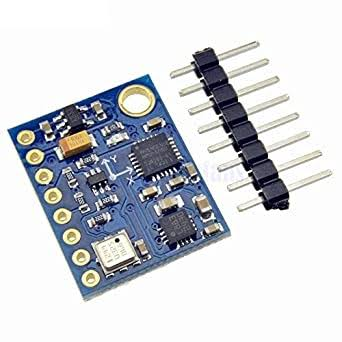
\includegraphics[width=0.25\textwidth]{imgs/gy87.png}
\caption{Mô-đun cảm biến GY-87 (MPU6050 + HMC5883L + BMP180).}
\label{fig:gy87}
\end{figure}

Dữ liệu bay được ghi lên thẻ microSD qua giao thức SPI. Bản mạch bố trí sẵn chỗ cho mô-đun vô tuyến Ai-Thinker Ra-02 (LoRa -- vô tuyến tầm xa, tốc độ thấp) -- phần mềm cho mô-đun này chưa được viết, là kết nối dự trữ cho nghiên cứu truyền thông ở giai đoạn tiếp theo. Ngoài ra còn có các connector phụ trợ MX1.25 cho bốn ESC, các khối I\textsuperscript{2}C1/UART/SPI/JTAG phục vụ mở rộng (UART: kênh truyền nối tiếp; JTAG: chuẩn gỡ lỗi phần cứng), hai nút bấm BOOT/RST, nút người dùng và LED RGB trạng thái.

\begin{figure}[h]
\centering
% Body cua Hinh 3.3 (fig:hw-block) -- chi chua tikzpicture, khong co preamble.
% \input tu 04_chapter4.tex (report chinh) va tu fig_preview/main.tex (render nhanh).
\begin{tikzpicture}[
  blk/.style={draw, thick, rounded corners=2pt, minimum height=0.8cm, inner sep=6pt, font=\footnotesize},
  pwr/.style={blk, fill=green!8, inner sep=5pt, align=center},
  mcu/.style={blk, fill=blue!10, text width=2.4cm, align=center, minimum height=1.6cm},
  per/.style={blk, fill=orange!12, text width=1.95cm, inner sep=4pt, align=center, minimum height=1.0cm},
  grp/.style={draw, thick, rounded corners=4pt, fill=gray!4},
  arr/.style={-{Stealth}, thick}
]
% ---------- Nu'a tren: cay nguon + MCU ----------
% Cot nguon vao (ben trai)
\node[pwr, text width=1.8cm] (bec) at (0.85,1.15) {BEC 5V (ESC)};
\node[pwr, text width=1.8cm] (lipo) at (0.85,0) {LiPo 1S};
\node[pwr, text width=1.8cm] (usb) at (0.85,-1.15) {USB-C 5V};
% Diode OR o giua: nguon tren vao tu bac, giu tu tay, nguoi tu nam
\node[pwr] (sel) at (3.5,0) {Diode OR 5V};
\draw[arr] (bec.east) -| (sel.north);
\draw[arr] (lipo.east) -- (sel.west);
\draw[arr] (usb.east) -| (sel.south);
% Duong chinh (AP2112K) o tren -> MCU; duong cam bien (ME6211) o duoi -> GY-87
\node[pwr, text width=2.0cm] (ap21) at (7.35,1.35) {AP2112K-3.3\\ +3V3 (chính)};
\node[pwr, text width=2.0cm] (me61) at (7.35,-1.35) {ME6211C33\\ +3V3\_SENS};
\coordinate (tk) at (5.05,0);
\draw[thick] (sel.east) -- (tk);
\draw[arr] (tk) |- (ap21.west);
\draw[arr] (tk) |- (me61.west);
\node[mcu] (mcu) at (10.7,0) {ESP32-S3\\WROOM-1\\2 $\times$ LX7\\240 MHz};
\draw[arr] (ap21.east) -| (mcu.north);
% ---------- Nu'a duoi: nhom ngoai vi ----------
\node[grp, minimum width=13.98cm, minimum height=2.0cm] (grpbox) at (8.49,-4.2) {};
\node[per, text width=1.85cm] (p1) at (2.81,-4.2) {microSD\\(SPI)};
\node[per, text width=1.85cm] (p2) at (5.08,-4.2) {4 $\times$ ESC\\(PWM\\250~Hz)};
\node[per, text width=1.85cm] (gy) at (7.35,-4.2) {GY-87\\(I\textsuperscript{2}C)};
\node[per, text width=1.85cm] (p4) at (9.62,-4.2) {FS-iA6B\\(PPM/RMT)};
\node[per, text width=1.85cm] (p5) at (11.89,-4.2) {RA-02 LoRa\\(SPI, dự trữ)};
\node[per, text width=1.85cm] (p6) at (14.16,-4.2) {WS2812\\USB-C\\nút bấm};
\draw[arr] (mcu.south) -- (grpbox.north -| mcu.south);
\draw[arr] (me61.south) -- (gy.north);
\end{tikzpicture}

\caption{Sơ đồ khối phần cứng \textbf{FC-v01} v2. Màu xanh lá: các khối nguồn (ba nguồn vào, diode OR và hai LDO). Màu xanh dương: khối xử lý trung tâm. Màu cam: nhóm ngoại vi. LDO ME6211C33 cấp riêng đường +3V3\_SENS cho GY-87; LDO AP2112K-3.3 cấp đường +3V3 chính cho toàn bộ các khối còn lại.}
\label{fig:hw-block}
\end{figure}
